%!TEX root = LiteratureReview.tex

\section{Quasi-Probability Distributions}
Probability distributions in the classical theory of probability are subject to 3 important restrictions, which derive from the Kolmogorov axioms on the system probability measure. The transition to a quantum theory of probability relaxes one or more of these axioms, and quasi-probability distributions result-these are not necessarily everywhere positive, and regions integrated under such distributions do not in general represent mutually exclusive states as do the analogous regions under true probability distributions. This corresponds to the relaxation of the first and third of Kolmogorov's axioms. 

Several different quasi-probability distribution representations are possible\autocite{Walls2008}, and to each is associated a theorem known as the \emph{Optical equivalence theorem} \autocite{Sudarshan1963}, for a power series of annihilation and creation operators in a given ordering. The optical equivalence theorem is concisely stated as follows
\begin{equation}
	\langle g_{\Omega} (\alpha, \alpha^*) \rangle = \langle g_{\Omega} (\hat{a}, \cre) \rangle
\end{equation}
with $g_\Omega$ some power series of $\hat{a}$ and $\cre$, and $\Omega$ the ordering of that power series. That is to say, the expectation of a power series of the operators $\hat{a}$ and $\cre$ is the same as the expectation value of the same power series with annihilation and creation operators replaced by complex eigenvalues $\alpha$ and $\alpha^*$ respectively, with regard to the appropriate quasiprobability distribution for that operator ordering. The quasiprobability distributions for each ordering are listed below.

Quasi-probability distributions arise naturally when considering representations of the density operator. The density operator is in general defined with regards to a complete orthonormal set of projection operators. However, a diagonal representation of the density operator in terms of an \emph{overcomplete} set of non-orthogonal projectors is also always possible \autocite{Sudarshan1963}, and the corresponding representation is in certain systems conceptually and computationally simpler. The relevant overcomplete set in quantum optics is the set of coherent states of the electromagnetic field defined as the right eigenstates of the annihilation operator
\begin{equation}
\alpha | \alpha \rangle = \ann | \alpha \rangle
\end{equation}
\subsection{Normal Ordering}
An operator ordering is \emph{normal} if in all products of annihilation and creation operators, all creation operators come before annihilation operators \autocite{Mandl2010} The Glauber-Sudarshan P function\autocite{Cahill1969}:
\begin{equation}
	\dens = \int P(\alpha) | \alpha \rangle \langle \alpha | d^2 \alpha
	\end{equation}
where $d^2 \alpha = dRe\{\alpha \}dIm\{\alpha \}$, is used for evaluating expectations of normally ordered power series:
\begin{equation}
	\langle \hat{a}^{\dagger n} \hat{a}^{m}  \rangle = \int \alpha^n \alpha^m P (\alpha, \alpha^*) d^2 \alpha
\end{equation}
P ($\alpha$) does not in general admit an interpretation as a classical probability distribution. However, the transition between quantum and classical systems is most clearly visible in the P representation; any system with a classical analogue (a coherent state, a chaotic state) has a non-negative, classically interpretable P function, and any with no classical analogue (Fock states, or states exhibiting squeezing, antibunching) will have a P function which is either negative or more singular than delta function. This statement is not generally true for other quasiprobability distributions\autocite{Mandel1995}
\subsubsection{General procedure for evaluating P ($\alpha$)}
\label{mehta}
There exists a general expression for evaluating the P-function that yields a well-behaved function whenever such a function is possible.\autocite{Mehta1967}:
\begin{equation}
	P(\alpha) = \frac{1}{\pi^2} \int d^2 \beta \bra{-\beta} \dens \ket{\beta} e^{|\beta|^2} e^{\beta^* \alpha -\alpha^* \beta}
\end{equation}
It is a necessary and suffient condition for this expression for P ($\alpha$) to be standard function that the function $ \bra{\beta} \dens \ket{\beta} e^{|\beta|^2} $ be square integrable. Should it not be square integrable P ($\alpha$) can only be understood in the context of generalised function theory.
\subsection{Antinormal Ordering}
\emph{Antinormal} ordering is the inverse of normal ordering, in that annihilation operators appear before creation operators. The associated quasi-probability distribution is the \emph{Husimi-Q Function} \autocite{Husimi1940}, defined as the diagonal matrix elements of the density operator in a pure coherent state
\begin{equation}
	Q = \frac{\langle \alpha | \dens | \alpha \rangle}{\pi}
	\label{qdef}
\end{equation}
The Q function is a nonnegative, the density function being a positive operator. It is also bounded above 
\begin{equation}
	Q \leq \frac{1}{\pi}
\end{equation}
Antinormally ordered expectation values can be evaluated as follows:
\begin{equation}
	\langle \hat{a}^n \hat{a}^{\dagger m}  \rangle = \int \alpha^n \alpha^m Q (\alpha, \alpha^*) d^2 \alpha
\end{equation}
The Q function exists for states which admit no P representation, and unlike the P or W function is always positive
\subsection{Symmetric Ordering}
The first quasi-probability distribution to be introduced and the most popular in the literature is the \emph{Wigner Function} \autocite{Wigner1932}, which satisfies the OET for symmetrically ordered products: those of the form $\frac{\ann \cre + \cre \ann}{2}$

True probability distributions for generalised position and momentum are only possible independently $\rho(x) = |\braket{x}{\psi}|^2$, $\rho(p) = |\braket{p}{\psi}|^2$. This is fundamental principle of quantum mechanics. A joint statistical treatment is however available through the Wigner quasi-probability distribution
\begin{equation}
	W(X_1, X_2) = \frac{1}{4 \pi} \int_{-\infty}^\infty dX e^{\frac{-iXX_2}{2}} \bra{X_1+X} \dens \ket{X_1-X}
\end{equation}
Expressed in terms of the generalised position and momentum in quantum optics: the field quadratures defined $\alpha = X_1 + iX_2$. Integrating over either quadrature yields the true probability distribution in the other quadrature.

The Wigner function is defined as the \emph{Wigner transform} of the density matrix, a general invertible transformation taking operators to functions on phase space. Its inverse, the \emph{Weyl transform}, returns functions to operators. The phase space formulation of quantum mechanics in its original form involves propagating such functions in time using Moyal's Evolution Equation \autocite{Curtright2011}. This same formalism is equivalently applied  through different integral transforms to the other representations.
\subsection{Characteristic Functions}
The above functions are equivalently derived from the antinormal, normal, and symmetric characteristic functions, defined as follows:
\begin{align}
	\chi_{A} (\eta) &= tr\{\dens e^{-\eta^* \hat{a}}e^{\eta \cre } \} \\
	\chi_{N} (\eta) &= tr\{\dens e^{\eta \cre}e^{-\eta^* \hat{a} } \} \\
	\chi_{S} (\eta) &= tr\{\dens e^{\eta^* \hat{a}-\eta \cre } \} 
\end{align}
with the corresponding quasiprobability distributions retrieved as the inverse Fourier transform of the corresponding characteristic function
 \begin{equation}
 	\{P|Q|W\} = \hat{\mathscr{F}}^{-1} [\chi_{\{N|A|S\}}]
\end{equation}
The existence of the inverse transform is necessary condition for the existence of a particular representation in terms of non-generalised functions. 
\subsection{Coherent State Representations}
The form of the density matrix for a system in pure coherent state $ | \alpha_0 \rangle $  is:
\begin{equation}
 	\dens = | \alpha_0 \rangle \langle \alpha_0 | 
 \end{equation}
 \subsubsection{P-function}
 From the properties of the delta function, the form of the P-function is evident:
\begin{equation}
	P(\alpha) = \delta^2(\alpha-\alpha_0)
\end{equation}
\subsubsection{Q-function}
The Q-function is evaluated through its definition \cref{qdef}:
\begin{equation}
	Q(\alpha) = \frac{\langle \alpha | \alpha_0 \rangle \langle \alpha_0 | \alpha \rangle}{\pi} = \frac{{|\langle \alpha | \alpha_0 \rangle |}^2}{\pi} =  \frac{e^{-{|\alpha_0 - \alpha |}^2}}{\pi}
\end{equation}
\subsubsection{Wigner Function}
The Wigner function is recovered from the Wigner transform of $\ket{\alpha_0}\bra{\alpha_0} = \ket{X_1+iX_2}\bra{X_1+iX_2}$
\begin{equation}
	W(x_1, x_2) = \frac{2}{ \pi} e^{-\frac{1}{2}[{(x_1-X_1)}^2+{(x_2-X_2)}^2]}
\end{equation}
\begin{figure}[h]
	\begin{minipage}[b]{.5\linewidth}
		\centering \large 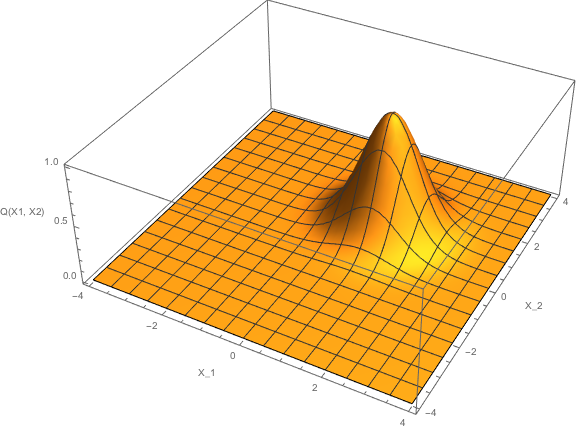
\includegraphics[width=1\textwidth]{Images/Q Function-Coherent.png} 
		\subcaption{W function for the Coherent state $\alpha=1+i$}\label{fig:Qcoh}
	\end{minipage}%
	\begin{minipage}[b]{.5\linewidth}
		\centering\large 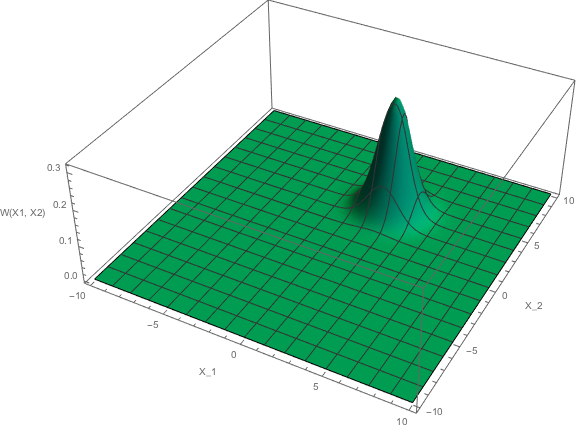
\includegraphics[width = 1\textwidth]{Images/W Function-Coherent.png}
		\subcaption{Q function for the Coherent state $\alpha=2+4i$}\label{fig:Wcoh}
	\end{minipage}
	% \caption{Coherent State Representations}\label{Coherents}
\end{figure}
\subsection{Fock state representations}
\subsubsection{P-function}
Since Fock states have no classical analogue, we would expect the P function associated with the Fock state density matrix $\ket{n}\bra{n}$ should be highly singular or negative. From \cref{mehta}, P ($\alpha$) is non-singular (not more singular than a $\delta$-function) if and only if $ \bra{\beta} \dens \ket{\beta} e^{|\beta|^2} $ is square integrable. But, using the Fock state expansion of the coherent states
\begin{align}
	 \bra{\beta} \dens \ket{\beta} e^{|\beta|^2}  &= e^{-|\beta|^2} \sum_{k=0}^\infty \frac {{\beta^*}^k}{k!} \braket{k}{n}\braket{n}{k} \sum_{k=0}^\infty \frac {\beta^k}{k!}e^{|\beta|^2} \\ &= e^{-|\beta|^2} \frac{|\beta|^{2n}}{{n!}^2} e^{|\beta|^2} \\ &= \frac{|\beta|^{2n}}{{n!}^2}
\end{align}
Which is square integrable for no value of n.
A representation in terms of a class of generalised functions called \emph{tempered distributions} is possible\footnote{Specifically, in terms of the derivatives of a Dirac delta function\autocite{Gerry2005}}, but the behaviour of such objects makes them difficult to work with.
\subsubsection{Q-function}
Despite the pathological nature of the Fock state P-function the Q-function is quite straightforwardly evaluated from its definition
\begin{align}
	 Q(\alpha) = \bra{\alpha} \dens \ket{\alpha}  &= \sum_{k=0}^\infty \frac {{\alpha^*}^k}{k!} \braket{k}{n}\braket{n}{k} \sum_{k=0}^\infty \frac {\alpha^k}{k!}e^{-|\alpha|^2} \\ &= \frac{|\alpha|^{2n}}{{n!}^2} e^{-|\alpha|^2}
\end{align}
\begin{figure}[h]
	\begin{minipage}[b]{.5\linewidth}
		\centering \large 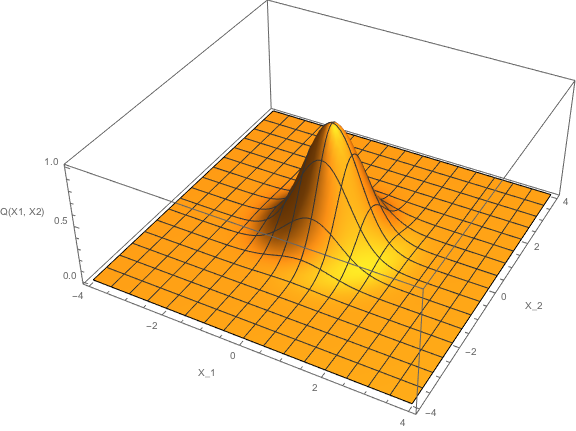
\includegraphics[width=1\textwidth]{Images/Q Function-n=0.png} 
		\subcaption{n=0}\label{fig:Qn=0}
	\end{minipage}%
	\begin{minipage}[b]{.5\linewidth}
		\centering\large 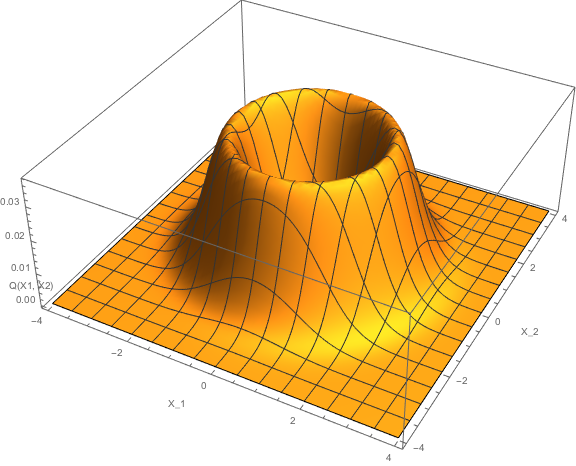
\includegraphics[width = 1\textwidth]{Images/Q Function-n=3.png}
		\subcaption{n=5}\label{fig:Qn=5}
	\end{minipage}
	\caption{Fock State Q Functions}\label{Qfunctions}
\end{figure}
\subsubsection{Wigner function}
The Wigner transform of $\ket{n}\bra{n}$ is\autocite[65]{Walls2008}
\begin{equation}
	W(x_1, x_2) = \frac{2}{\pi} {(-1)}^n \mathscr{L}_n(4(x_1^2+x_2^2))e^{-2(x_1^2+x_2^2)}
\end{equation}
Where $\mathscr{L}_n$ is the nth Laguerre Polynomial.
\begin{figure}[h]
	\begin{minipage}[b]{.5\linewidth}
		\centering \large 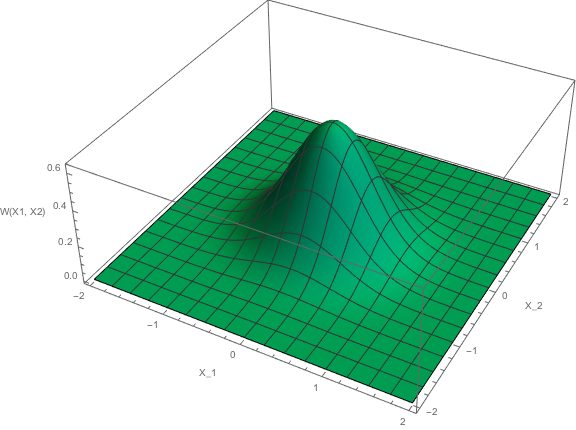
\includegraphics[width=1\textwidth]{Images/W Function-n=0.png} 
		\subcaption{n=0}\label{fig:n=0}
	\end{minipage}%
	\begin{minipage}[b]{.5\linewidth}
		\centering\large 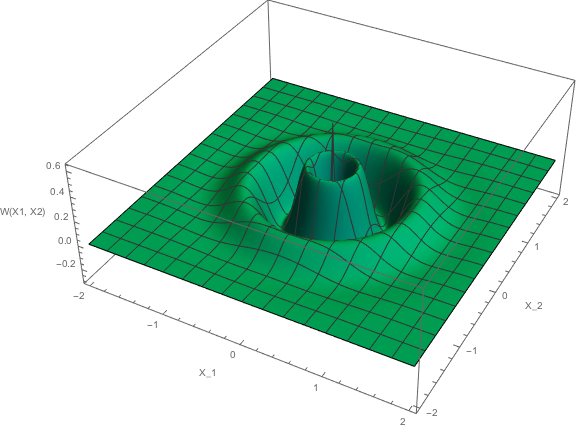
\includegraphics[width = 1\textwidth]{Images/W Function-n=10.png}
		\subcaption{n=10}\label{fig:n=10}
	\end{minipage}
	\caption{Fock State Wigner Functions}\label{Wfunctions}
\end{figure}


